The Damage and Loss panel provides users a convenient way to define the damage and loss model for the building. The dropdown list at the top of the panel allows users to choose between two loss-assessment methods: FEMA P58 \cite{applied_technology_council_atc_fema_2012} and HAZUS MH \cite{federal_emergency_management_agency_fema_hazus_2018-2}. The method chosen determines the information displayed in the rest of the panel. The two methods are discussed in the following sections.

\subsection{FEMA P58}

This option implements the loss assessment methodology described in the \href{https://www.fema.gov/media-library/assets/documents/90380}{FEMA P58} documents. The main panel is divided into three parts that can be accessed by clicking at the tabs at the top of the input panel.

\subsubsection{General Settings}

\Cref{fig:dl_p58_general} shows the first panel, which corresponds to general settings. The panel allows the user to define the response, damage, and loss model and the dependencies between model parameters. Each setting is described in detail below.

\begin{figure}[!htbp]
  \centering {
    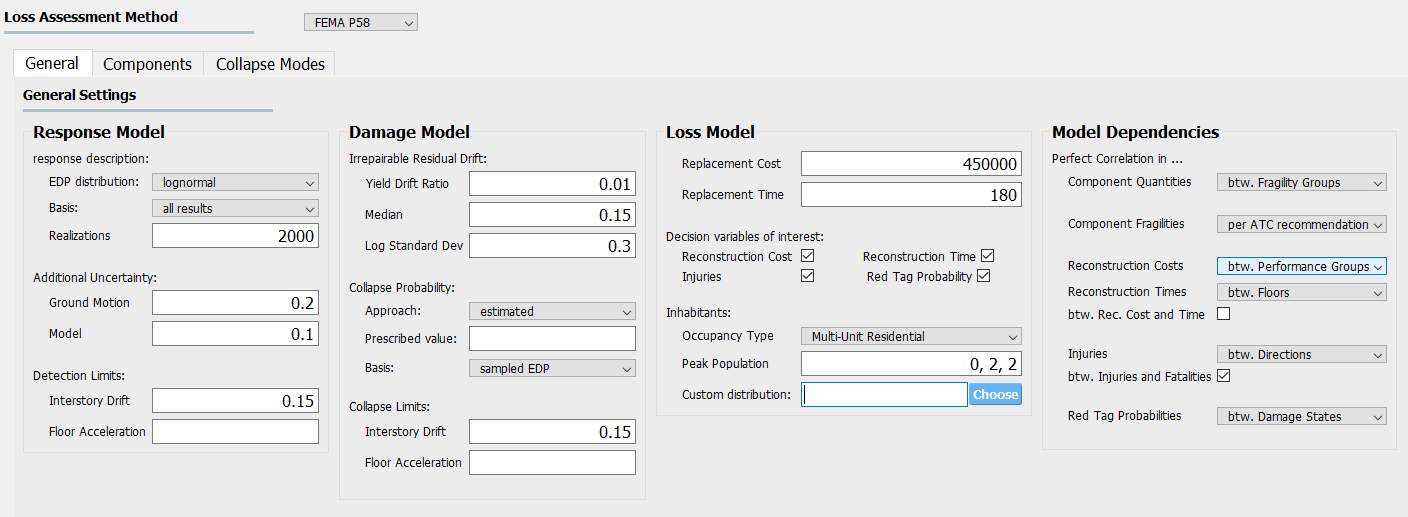
\includegraphics[width=1.1\textwidth]
    {usage/figures/dl_p58_general.png} }
  \caption{The General Damage and Loss Settings panel. (The settings shown in the Figure serve demonstration purposes and are not the suggested inputs.)}
  \label{fig:dl_p58_general}
\end{figure}

\textbf{Response Model}

\begin{itemize}
    \item Response Description
    \begin{itemize}
        \item EDP distribution\\
        When running multiple response simulations, the resulting set of EDP samples describe the uncertainty in the estimated response. We provide three options to use these samples: i) if the  \textit{empirical} option is chosen, the EDP data is used as-is, no distribution is assigned to the EDPs; ii) in the \textit{lognormal} case we fit a multivariate lognormal distribution to the EDP samples; iii) while in the \textit{truncated lognormal} case we fit a truncated multivariate lognormal distribution to the samples. The truncation limits are defined by the Collapse limits under the Damage model.
        \item Basis\\
        Specifies which part of the EDP data shall be used to estimate the EDP distribution. This information is only required if the EDP distribution is set to lognormal. The \textit{all results} option uses every available EDP sample, while the \textit{non-collapse results} option discards the collapsed cases (i.e., EDPs above the collapse limits).
        \item Realizations\\
        The number of realizations to generate using the stochastic loss model. Depending on the complexity of the model, a few thousand realizations might be sufficient to capture central tendencies. A much larger number is required to get appropriate estimates of the dispersion of results.
    \end{itemize}
    \item Additional uncertainty\\
    Ground motion and modeling uncertainty per FEMA P58. The prescribed logarithmic standard deviation values are added to the dispersion of EDPs to arrive at the description of uncertain building response. Additional uncertainty is not considered when the empirical EDP distribution option is selected.
    \item Detection Limits\\
    These limits correspond to the maximum possible values that the response history analysis can provide. While peak interstory drifts will certainly have an upper limit, peak floor acceleration will not necessarily require such a setting. Leaving any of the fields empty corresponds to unlimited confidence in the simulation results.\\
    Note: these limits will be used to consider EDP data as a set of censored samples when fitting a distribution to simulation results. Detection limits are not considered when the empirical EDP distribution option is selected.
\end{itemize}

\textbf{Damage Model}

\begin{itemize}
    \item Irrepairable Residual Drift
    \begin{itemize}
        \item Yield Drift Ratio\\
        This prescribed value is used to estimate residual drifts from peak interstory drifts per Section 5.4 in FEMA P58. These are only needed if no reliable residual drifts are available from the simulation. Considering the large uncertainty in estimated residual drift values, it is recommended to consider using the peak interstory drift as a proxy even if it would be numerically possible to obtain residual drift values.
        \item Median and Log Std\\
        Describes the limiting residual drift as a random variable with a Lognormal distribution. See Figure 2-5 and Section 7.6 in FEMA P58 for details.
    \end{itemize}
    \item Collapse Probability
    \begin{itemize}
        \item Approach\\
        Specifies the approach to determine the probability of collapse. If \textit{estimated} is chosen, the collapse probability is determined based on the Collapse limits (see below) and the EDP samples. If \textit{prescribed} is chosen, a user-defined collapse probability is used. This is useful, for example, if the PBE App is used to perform a series of scenario calculations for a time-based assessment and the user prefers to apply a collapse fragility function to control the probability of collapse at each investigated scenario.
        \item Prescribed value\\
        The user-defined probability of collapse; only used if the approach above is set to prescribed. The prescribed value shall be between 0.0 and 1.0.
        \item Basis\\
        Specifies the data that shall be used to estimate the collapse probability. This setting is only used if the approach above is set to estimated. If the \textit{raw EDP} option is chosen, the raw data from response simulation is used and the probability of collapse is defined as the number of samples above the collapse limits over the total number of samples. If the \textit{sampled EDP} is chosen, the prescribed number of realizations are sampled from the EDP distribution and these samples are used to estimate the probability of collapse.
    \end{itemize}
    \item Collapse Limits\\
    The collapse limits describe the EDP value beyond which the building is considered collapsed. Note that collapse limits might be beyond the detection limits (although that is generally not a good idea) and certain EDPs might not have collapse limits associated with them (e.g. PFA).
\end{itemize}

\textbf{Loss Model}

\begin{itemize}
    \item Replacement Cost and Time\\
    The cost (in the currency used to describe repair costs, typically US dollars) and the time (in days) it takes to replace the building.
    \item Decision Variables of interest\\
    These checkboxes allow the user to pick the decision variables of interest and save computation time and storage space by only focusing on those. Expect this list to grow as more decision variables are added in the future.
    \item Inhabitants
    \begin{itemize}
        \item Occupancy type\\
        The type of occupancy is used to describe the temporal distribution of the inhabitants. Note: the default FEMA P58 distribution can be overridden by a custom file provided in the Custom Data Sources box.
        \item Peak Population\\
        The maximum number of people present at each floor of the building provided as a comma-separated list. If only one value is provided, we assign that as the peak population for every floor. The example in \Cref{fig:dl_p58_general} shows a two-story wooden house with a cripple wall, hence the 0 population in the first floor.
        \item Custom distribution\\
        By default, the loss assessment is performed using population and fragility data from the first edition of FEMA P58. This field allows the user to define a custom distribution for the population over time (24h ,weekday/weekend, and months of the year).\\
        Note: the loss calculations are performed at the local computer. Consequently, the locally available fragility and population data files do not need to be shared with the community, and they can be used to perform the calculations even if the response simulations are done at DesignSafe.
    \end{itemize}
\end{itemize}

\vspace{12pt}
\textbf{Model Dependencies}
\vspace{6pt}

The PBE App allows you to specify dependencies between various parts of the loss model. The default FEMA P58 setting assumes all variables are independent, except for the fragility data, where the fragility of certain Component Groups (i.e. groups of components with identical behavior within Performance Groups) is perfectly correlated. This behavior is achieved by setting every other dependency to Independent and setting the Component Fragilities to \texttt{per ATC recommendation}. This is the default configuration in the PBE App.
Every type of prescribed dependency assumes perfect correlation between a subset of the loss model’s variables and no correlation between others. If there is interest in the research community, future versions will expand on this approach by introducing more complex correlation structures.
Perfect correlation can be assigned between the following logical components of the model:

\begin{itemize}    
    \item Fragility Groups\\
    Assumes that the selected parameters are correlated between Fragility Groups (i.e. the highest organizational level) and at every level below. With this setting, the user assigns perfect correlation between every single parameter of the selected type in the model. Use this with caution.
    \item Performance Groups\\
    Assumes that the selected parameters are correlated between all Performance Groups and at every logical level below. For instance, this setting for Component Quantities will lead to identical deviations from mean quantities among the floors and directions in the building.
    \item Floors\\
    Assumes that the selected parameters are correlated between Performance Groups at various floors, but not between Performance Groups in different directions in the building. Also assumes perfect correlation between the Damage States within each Performance Group. This is useful when the parameter is direction-dependent and similar deviations are expected among all floors in the same direction.
    \item Directions\\
    Assumes that the selected parameters are correlated between Performance Groups in various (typically two) directions, but not between different floors of the building. This can be useful when you want to prescribe similar deviations from mean values within each floor, but want to allow independent behavior over the height of the building.
    \item Component Groups\\
    Assumes that the selected parameters are correlated between Component Groups. This will set parameters of components within a Performance Group perfectly correlated, but keep the different Performance Groups independent.
    \item Damage States\\
    Correlation at the lowest organizational level. Assumes that the selected parameters are correlated between Damage States only. This type of correlation, for instance, would assume that deviation from the median reconstruction cost is due to factors that affect all types of damage within a performance group in identical fashion.
\end{itemize}

The following model parameters can handle the assigned dependencies:

\begin{itemize}
    \item Component Quantities\\
    The amount of components in the building (see the description of the Components tab below for more details).
    \item Component Fragilities\\
    Each Damage State has a corresponding random EDP limit. The component fragilities is a collection of such EDP limit variables.\\
    Note: most methodologies assume that such EDP limits are perfectly correlated at least among the Damage States within a Component Subgroup.
    \item Reconstruction Costs and Times\\
    The cost and time it takes to repair a particular type of damage to a component. The btw. Rec. Cost and Time checkbox allows you to define correlation between reconstruction cost and time on top of the correlations already set above for each of these individually. \\
    Note: if you do define such a correlation structure, the more general correlation among the settings in the Reconstruction Costs and Reconstruction Times lines will need to be applied to both cases to respect conditional correlations in the system. (e.g., if you set costs to be correlated between Performance Groups and times to correlate between Floors and check the cost and time correlation as well, times will be forced to become correlated between Performance Groups.)
    \item Injuries\\
    The probability of being injured at a given severity when being in the affected area of a damaged component. Note that the Injuries lines prescribe correlations between the same level of injury at different places in the building. Correlation between different levels of injury at the same place can be prescribed by the btw. Injuries and Fatalities checkbox.
    \item Red Tag Probabilities\\
    The amount of damage in a given Damage State that triggers an unsafe placard or red tag.
\end{itemize}

\subsubsection{Building Components}

\Cref{fig:dl_p58_comp} shows the input panel used to define the components of the building. First, the set of building components is defined in the \textit{Component Selection} box, then the component attributes are set under \textit{Component Details}. The \textit{Component Input Overview} provides a glance at the provided attributes and allows the user to spot missing attributes or incorrect settings.

\begin{figure}[!htbp]
  \centering {
    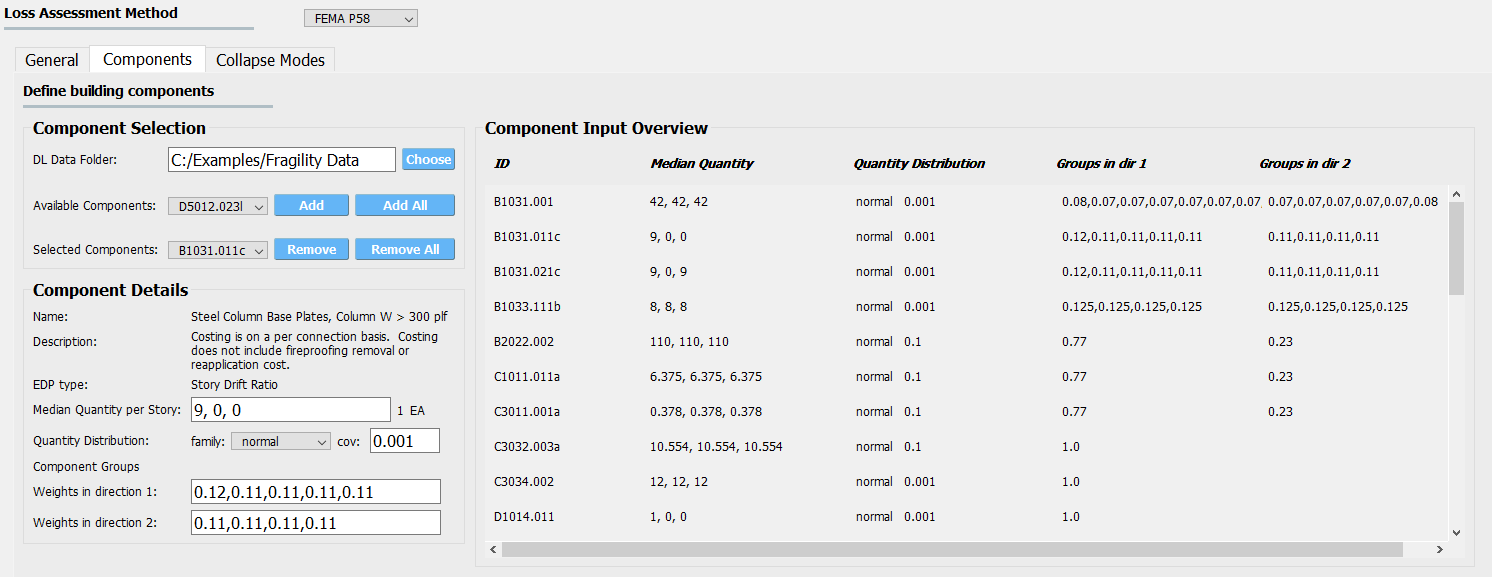
\includegraphics[width=1.1\textwidth]
    {usage/figures/dl_p58_comp.png} }
  \caption{The Building Components panel. (The settings shown in the Figure serve demonstration purposes and are not the suggested inputs.)}
  \label{fig:dl_p58_comp}
\end{figure}

\vspace{12pt}
\textbf{Component Selection}
\vspace{6pt}

The available components are loaded from the default component database compiled from the first edition of FEMA P58. Other, user-defined, custom components can be included either by adding component data files to the default database (located in the applications/performDL/resources folder) or by changing the location of DL data using the \textit{DL Data Folder} option in the upper left corner of the input panel. We recommend using the custom folder option to include user-defined components.\\
Note: the loss calculations are performed at the local computer. Consequently, the locally available component data files do not need to be shared with the community, and they can be used to perform the calculations even if the response simulations are done at DesignSafe.

Once the available set of components is defined, the user can add components to the building by clicking on the \textit{Add} button. The \textit{Add All} button adds every component from the available set to the analysis. This is often helpful when the custom component folder contains a selection of component files for a particular building. The \textit{Remove} and \textit{Remove All} buttons remove one or all components from the selected set, respectively.

\vspace{12pt}
\textbf{Component Details}
\vspace{6pt}

Once a component is selected in the \textit{Selected Components} drop-down menu, its attributes can be set here. Using the component data files, the following pieces of information are automatically displayed for each component:

\begin{itemize}
    \item ID: The ID of the component is the ID used in FEMA P58 and in PACT. This is also the name of the \texttt{json} file that contains the component data in the component data folder. When introducing custom components they shall have a unique ID and the corresponding file has to be renamed accordingly.
    Note: The ID does not have to follow the FEMA P58 naming convention.
    \item Name\\
    A brief description of the component.
    \item Description\\
    A more detailed description of the component.
    \item EDP type\\
    Specifies the type of EDP the component fragilities are based on. The types of EDPs are either Story Drift Ratio or Peak Floor Acceleration in the default FEMA P58 database, but user-defined components are allowed to use any other EDP types as long as the response estimation can provide such results for loss assessment.
\end{itemize}

The following component attributes need to be defined by the user:

\begin{itemize}
    \item Median Quantity per Story\\
    A list of median component quantities on each floor of the building. The quantities shall be specified in the units assigned to the component in the fragility data file. Those units are displayed by the input field for convenience.
    \item Quantity Distribution\\
    The random distribution family and the coefficient of variation used to define the uncertainty in component quantities.
    \item Component Groups\\
    Components within a Fragility Group are separated into Performance Groups by floor and direction. Components within a Performance Group are further separated into Component Groups that might experience independent damage and losses depending on the settings in the General tab. The weights defined for each direction specify the Component Groups in each floor. The same weight pattern is applied to all floors of the building. The weights shall sum to one.
\end{itemize}

\subsubsection{Collapse Modes}

\Cref{fig:dl_p58_collmod} shows the input panel where you can specify the collapse modes of the building. Collapse modes provide information for the estimation of injuries from building collapse. As such, they are only used if injuries are among the requested Decision Variables. The following pieces of information are required for each collapse mode:

\begin{figure}[!htbp]
  \centering {
    \includegraphics[width=0.6\textwidth]
    {usage/figures/dl_p58_collmod.png} }
  \caption{The Collapse Modes panel. (The settings shown in the Figure serve demonstration purposes and are not the suggested inputs.)}
  \label{fig:dl_p58_collmod}
\end{figure}

\begin{itemize}
    \item name: A name that helps you identify the collapse mode. It is arbitrary and not used by the loss assessment engine.
    \item probability: Conditioned on collapse, the likelihood of this collapse mode.
    \item affected area: The affected area (as a fraction of the total plan area) of the building at each floor. We assume that the floor area is uniform along the height of the building.
    \item injuries: The probability of each level of injury when people are in the affected area and this collapse mode occurs. (FEMA P58 assumes two levels of severity: injuries and fatalities).
\end{itemize}

\subsection{HAZUS MH}

This option implements the loss assessment methodology described in the \href{https://www.fema.gov/media-library-data/20130726-1820-25045-6286/hzmh2_1_eq_tm.pdf}{HAZUS MH Technical Manual} document. \Cref{fig:dl_hazus_general} shows the input panel that allows the user to define the response, damage, and loss model. Each setting is described in detail below.

\begin{figure}[!htbp]
  \centering {
    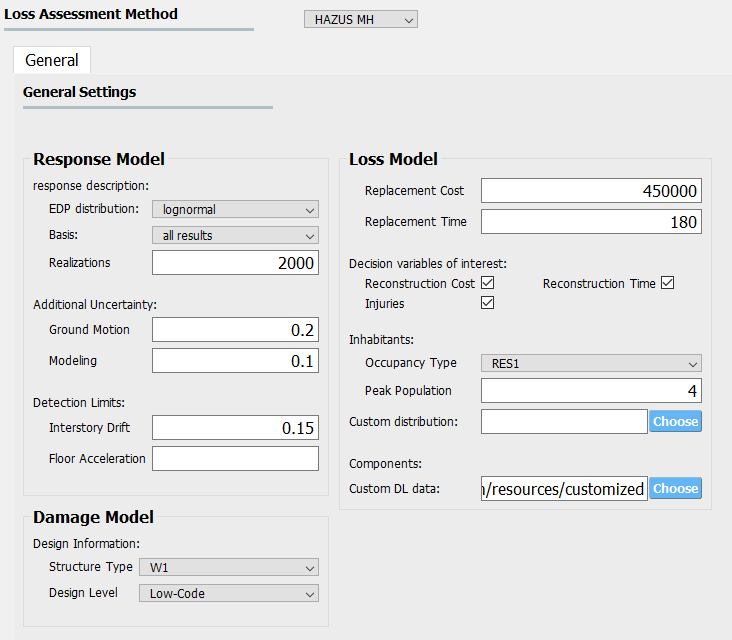
\includegraphics[width=0.7\textwidth]
    {usage/figures/dl_hazus_general.png} }
  \caption{The General Damage and Loss Settings panel. (The settings shown in the Figure serve demonstration purposes and are not the suggested inputs.)}
  \label{fig:dl_hazus_general}
\end{figure}

\textbf{Response Model}

\begin{itemize}
    \item Response Description
    \begin{itemize}
        \item EDP distribution\\
        When running multiple response simulations, the resulting set of EDP samples describe the uncertainty in the estimated response. We provide three options to use these samples: i) if the  \textit{empirical} option is chosen, the EDP data is used as-is, no distribution is assigned to the EDPs; ii) in the \textit{lognormal} case we fit a multivariate lognormal distribution to the EDP samples; iii) while in the \textit{truncated lognormal} case we fit a truncated multivariate lognormal distribution to the samples. The truncation limits are defined by the Collapse limits under the Damage model.
        \item Basis\\
        Specifies which part of the EDP data shall be used to estimate the EDP distribution. This information is only required if the EDP distribution is set to lognormal. The \textit{all results} option uses every available EDP sample, while the \textit{non-collapse results} option discards the collapsed cases (i.e., EDPs above the collapse limits).
        \item Realizations\\
        The number of realizations to generate using the stochastic loss model. Depending on the complexity of the model, a few thousand realizations might be sufficient to capture central tendencies. A much larger number is required to get appropriate estimates of the dispersion of results.
    \end{itemize}
    \item Additional uncertainty\\
    Ground motion and modeling uncertainty per FEMA P58 that is referred to as uncertainty in response due to variability of ground motion demand and variability in the capacity properties of the model building in HAZUS MH. The prescribed logarithmic standard deviation values are added to the dispersion of EDPs to arrive at the description of uncertain building response.
    \item Detection Limits\\
    These limits correspond to the maximum possible values that the response history analysis can provide. While peak interstory drifts will certainly have an upper limit, peak floor acceleration will not necessarily require such a setting. Leaving any of the fields empty corresponds to unlimited confidence in the simulation results.\\
    Note: these limits will be used to consider EDP data as a set of censored samples when fitting a distribution to simulation results. Detection limits are not considered when the empirical EDP distribution option is selected.
\end{itemize}

\textbf{Damage Model}

\begin{itemize}
    \item Design Information\\
    The Structure Type and the Design Level per HAZUS MH. These two pieces of information are used to select the appropriate fragility and consequence functions from those provided in the HAZUS MH Tehcnical Manual.\\
    Note: Any fragility or consequence function can be edited by the user and loaded by specifying a directory that contains those custom functions in the Custom Data Sources box.
\end{itemize}

\textbf{Loss Model}

\begin{itemize}
    \item Replacement Cost and Time\\
    The cost (in the currency used to describe repair costs, typically US dollars) and the time (in days) it takes to replace the building.
    \item Decision Variables of interest\\
    These checkboxes allow the user to pick the decision variables of interest and save computation time and storage space by only focusing on those. Expect this list to grow as more decision variables are added in the future.
    \item Inhabitants
    \begin{itemize}
        \item Occupancy type\\
        The type of occupancy is used to describe the temporal distribution of the inhabitants. Note: the default HAZUS MH distribution can be overridden by a custom file provided in the Custom Data Sources box.
        \item Peak Population\\
        The maximum number of people present in the buildng. The example in \Cref{fig:dl_hazus_general} shows a single-family home with a total population of 4 people.
        \item Custom distribution\\
        By default, the loss assessment is performed using population distribution data from the HAZUS MH Technical Manual. This field allows the user to define a custom distribution for the population over time (24h ,weekday/weekend, and months of the year).
	\end{itemize}
	\item Components\\
	By default, the loss assessment is performed using component fragility data from HAZUS MH Technical Manual. This field allows the user to define custom component fragilities.\\
	Note: the loss calculations are performed at the local computer. Consequently, the locally available fragility and population data files do not need to be shared with the community, and they can be used to perform the calculations even if the response simulations are done at DesignSafe.
\end{itemize}